% Contributions are much appreciated, in order to contribute to this project, head over to this repository:
% https://github.com/bshramin/uofa-eng-assignment

\documentclass[11pt,letterpaper]{article}
\textwidth 6.5in
\textheight 9.in
\oddsidemargin 0in
\headheight 0in
\usepackage{graphicx}
\usepackage{fancybox}
\usepackage[utf8]{inputenc}
\usepackage{epsfig,graphicx}
\usepackage{multicol,pst-plot}
\usepackage{pstricks}
\usepackage{amsmath}
\usepackage{amsfonts}
\usepackage{amssymb}
\usepackage{eucal}
\usepackage[left=2cm,right=2cm,top=2cm,bottom=2cm]{geometry}
\usepackage{esvect}
\pagestyle{empty}
\DeclareMathOperator{\tr}{Tr}
\newcommand*{\op}[1]{\check{\mathbf#1}}
\newcommand{\bra}[1]{\langle #1 |}
\newcommand{\ket}[1]{| #1 \rangle}
\newcommand{\braket}[2]{\langle #1 | #2 \rangle}
\newcommand{\mean}[1]{\langle #1 \rangle}
\newcommand{\opvec}[1]{\check{\vec #1}}
\renewcommand{\sp}[1]{$${\begin{split}#1\end{split}}$$}

\usepackage{lipsum}

\usepackage{listings}
\usepackage{color}
\usepackage{wrapfig}
\usepackage[shortlabels]{enumitem}

\definecolor{codegreen}{rgb}{0,0.6,0}
\definecolor{codegray}{rgb}{0.5,0.5,0.5}
\definecolor{codepurple}{rgb}{0.58,0,0.82}
\definecolor{backcolour}{rgb}{0.95,0.95,0.92}

\lstdefinestyle{mystyle}{
	backgroundcolor=\color{backcolour},   
	commentstyle=\color{codegreen},
	keywordstyle=\color{magenta},
	numberstyle=\tiny\color{codegray},
	stringstyle=\color{codepurple},
	basicstyle=\footnotesize,
	breakatwhitespace=false,         
	breaklines=true,                 
	captionpos=b,                    
	keepspaces=true,                 
	numbers=left,                    
	numbersep=5pt,                  
	showspaces=false,                
	showstringspaces=false,
	showtabs=false,                  
	tabsize=2
}

\lstset{style=mystyle}

\begin{document}
\pagestyle{plain}

\begin{flushleft}
Estudiante: Fabio Quimbay\\
Email: fabio.quimbay883@comunidadunir.net\\
Profesor: Miguel Ángel Cabeza\\
Fecha: Noviembre 14 de 2022\\
\end{flushleft}

\begin{flushright}\vspace{-20mm}

\includegraphics[height=2cm]{logo.png}
\end{flushright}
 
\begin{center}\vspace{0cm}
\textbf{\large PER5786 2022-2023  Física 1 (GFI) - PER5786 2022-2023}\\
 Tema 4 - Dinámica - Leyes de Newton
\end{center}

 
\rule{\linewidth}{0.1mm}
%%%%%%%%%%%%%%%%%%%%%%%%%%%%%%%%%%%%%%%%%%%%%%%%%%%%%%%%%%%%%%%%%%%%%%%%

\bigskip
\bigskip

%%%%%%%%%%%%%%%%%%%%
\textbf{Problema propuesto 2}\\

\begin{wrapfigure}{r}{0.25\textwidth}
\begin{center}
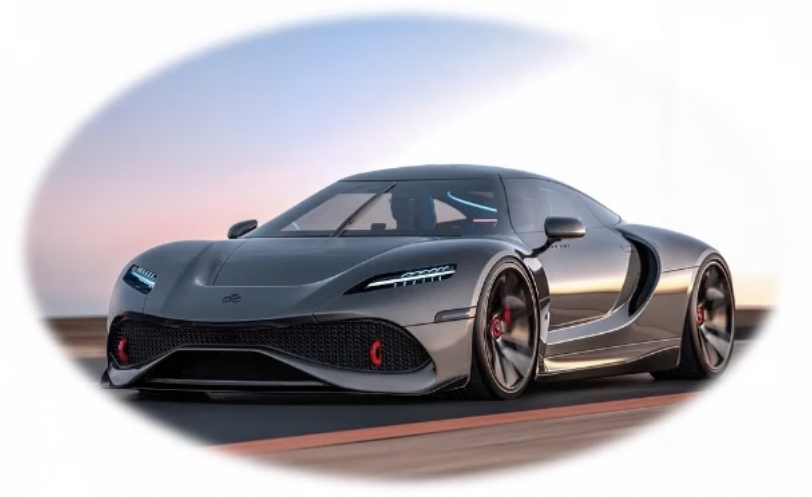
\includegraphics[width=0.25\textwidth]{problema_2.png}
\end{center}
\end{wrapfigure}

El viento actúa sobre un vehículo de 1000 kg con una fuerza de 100 N durante 10 s en sentido contrario a su velocidad. Calcula: a) La variación de la cantidad de movimiento del cuerpo. b) Su velocidad final si en el momento de actuar la fuerza, el vehículo se mueve a 100 m/s.\\

\textbf{Formulas base:}\\

Se tomarán las siguientes formulas base de la Dinámica Clásica (Leyes de Newton):

\begin{align}
\boxed{ \vec{F} = \frac{d\vec{p}}{dt} = \frac{d (m \vec{v})}{dt} = m \cdot \vec{a} }\\
\boxed{ 1\,N = 1\,Kg \cdot m/s^2}\\
\boxed{ \vec{P} = m \cdot \vec{g} }\\
\boxed{ \vec{F} = \frac{d\vec{p}}{dt} }
\end{align}

\textbf{Solución:}\\

De acuerdo a la ecuación (1) podemos despejar la variación de la cantidad de movimiento, asi:

\begin{align}
d\vec{p} = \vec{F_{auto}} \cdot dt = -100\,N \cdot 10\,s = -1000\,Kg \cdot m/s
\end{align}

Por otro lado, basado en la ecuación (1) se puede despejar la velocidad final ($V_{f}$) del automóvil, a saber:

\begin{align*}
V_{f_{auto}} &= V_{0_{auto}} + \frac{\vec{F_{auto}}}{m} \cdot (t_{f} - t_{0})\\
V_{f_{auto}} &= 100 + \frac{(-100)(10)}{1000\,kg}\\
V_{f_{auto}} &= 100 -1 = 99\,m/s\\
\end{align*}

La velocidad final del automóvil ($V_{f_{auto}}$) será de $99\,m/s.$

%%%%%%%%%%%%%%%%%%%%

\end{document}

